% Chương Mô hình dự đoán khách hàng rời bỏ
% Bảng m_*.tex và hình m_*.png do python/tao_bang_tex_mohinh.py sinh từ results/. Không sửa tay số liệu trong latex/bang/.
\section{Mô hình dự đoán khách hàng rời bỏ}

Chương này trả lời câu hỏi thứ nhất của đề tài: khách hàng nào có nguy cơ không mua lại. Đầu vào là bảng Customer Snapshot (Chương 3) và nhãn $y$ (Chương 4). Đầu ra là xác suất không mua lại của từng khách, gọi là \texttt{RiskScore}, được ghi vào kho để DSS ở Chương 6 dùng. Chương đi theo quy trình phân lớp hai bước của tài liệu môn học~\cite{tlmh}: học mô hình rồi dùng mô hình để dự đoán. Mọi con số lấy từ kết quả chạy trên kho \texttt{CompanyX\_DW}.

\subsection{Bài toán và tiêu chí chọn mô hình}
\subsubsection{Bài toán}
Đây là bài toán phân lớp hai lớp. Với mỗi khách tại mốc $T$, mô hình nhận các thuộc tính ở Bảng~\ref{tab:thuoctinh} và trả về xác suất $p$ của việc khách không mua lại trong 90 ngày tới ($y=1$). Nhóm cần xác suất chứ không chỉ cần nhãn, vì Chương 6 phải so lợi ích kỳ vọng của việc chăm sóc với chi phí bỏ ra. Hai khách cùng bị dự đoán không mua lại nhưng có xác suất 0,95 và 0,60 thì đáng đầu tư khác nhau.

\subsubsection{Giá trị ròng $Z$: tiêu chí kinh doanh}
Độ chính xác chưa cho biết mô hình có giúp giữ được tiền hay không. Vì vậy nhóm đo thêm giá trị ròng $Z$: số tiền kỳ vọng giữ lại được khi dùng điểm của mô hình để chọn khách chăm sóc trong một ngân sách cố định. Cách tính theo Chương 6: lợi nhuận gộp một đơn của khách $i$ là $v_i = g \cdot AOV_i$, với $AOV_i$ là tiền hàng trung bình mỗi đơn và $g = 41{,}15\%$ là tỷ lệ lợi nhuận gộp tính từ giá vốn. Giá trị kỳ vọng khi chăm sóc khách $i$ là
\begin{equation}
    EV_i = p_i \cdot r \cdot v_i - c
\end{equation}
với $r$ là tỷ lệ chăm sóc thành công và $c$ là chi phí chăm sóc một khách. Danh sách chọn gồm $K = \min(\lfloor B/c \rfloor,\ \text{số khách có } EV_i > 0)$ khách có $p_i v_i$ lớn nhất, với $B$ là ngân sách. Trên mốc đánh giá đã biết nhãn thật $y_i$, giá trị ròng là
\begin{equation}
    Z = r \sum_{i \in S} y_i v_i - c\,K
\end{equation}
với $S$ là danh sách đã chọn. Chỉ khách thật sự không mua lại đem lại lợi ích, vì khách vốn sẽ mua lại thì không cần chăm sóc.

Kịch bản cơ sở là $r = 10\%$, $c = 10$ USD và $B = 40.000$ USD, nên $K = 4.000$. Vì $r$ là giả định, $Z$ chỉ dùng để so các mô hình với nhau, không phải dự báo doanh thu. Hai mốc tham chiếu là chọn chỉ theo giá trị $v$ mà không dùng mô hình (trung bình bốn fold 269.043 USD) và chọn khi biết trước ai không mua lại (346.378 USD). Mô hình hữu ích phải nằm giữa hai mốc này, càng gần mốc sau càng tốt.

\subsubsection{Ba điều kiện chọn mô hình}\label{sec:chon}
Nhóm đặt trước ba điều kiện, mỗi điều kiện ứng với một cách nhìn về mô hình. Một mô hình chỉ được chọn khi đạt cả ba ở mọi fold.
\begin{enumerate}
    \item \textbf{ĐK1, xếp hạng:} ROC-AUC không thấp hơn quy tắc Recency đảo chiều. Cụ thể, khoảng tin cậy 95\% của hiệu hai ROC-AUC (bootstrap, tức lấy mẫu lại có hoàn lại 500 lần để ước lượng khoảng tin cậy~\cite{efron1993}) có cận trên không âm. ROC-AUC và Brier định nghĩa ở mục~\ref{sec:chisobosung}.
    \item \textbf{ĐK2, chất lượng xác suất:} Brier thấp hơn Brier của cách gán cùng một xác suất cho mọi khách.
    \item \textbf{ĐK3, giá trị quyết định:} $Z$ cao hơn $Z$ khi chỉ chọn theo giá trị $v$.
\end{enumerate}
Khi nhiều mô hình cùng đạt, nhóm chọn mô hình có $Z$ cao hơn ở nhiều mốc hơn.

\subsubsection{Các mô hình thử nghiệm}
Nhóm thử chín phương án với cấu hình cố định trước khi chạy (Bảng~\ref{tab:cacmohinh}). Naive Bayes và cây quyết định thuộc nội dung môn học~\cite{han2011}, cây dùng chỉ số Gini của CART~\cite{hastie2009}. Mạng nơ-ron (mục 2.3), Random Forest~\cite{breiman2001}, gradient boosting và kNN~\cite{hastie2009} ngoài nội dung môn học, được thử để biết giới hạn của dữ liệu. Hồi quy logistic và hai mốc so sánh cho biết mô hình chính hơn các cách đơn giản bao nhiêu.

\begin{table}[!htbp]
\centering
\caption{Các mô hình thử nghiệm và cấu hình cố định}
\label{tab:cacmohinh}
\footnotesize
\begin{tabular}{p{3.2cm}p{2.6cm}p{8.6cm}}
\toprule
Mô hình & Vai trò & Cấu hình \\
\midrule
Naive Bayes & Chấm điểm & Năm thuộc tính đã chia khoảng (Recency 6 khoảng, Frequency 3, Monetary 4 theo tứ phân vị, BikeBuyer 2, NSub 4), làm trơn Laplace với hệ số 1 \\
Cây quyết định Gini & Đối chứng, sinh luật & 11 thuộc tính, sâu tối đa 4, mỗi lá có ít nhất 400 khách, xác suất lá làm trơn với $m=50$ \\
Mạng nơ-ron MLP & So sánh & 11 thuộc tính chuẩn hoá z-score, hai tầng ẩn 32 và 16 nơ-ron, ReLU, dừng sớm, hạt giống 0 \\
Hồi quy logistic & So sánh & Năm thuộc tính đã chia khoảng, mã hoá one-hot (mỗi khoảng thành một cột 0/1), chính quy hoá L2 \\
Luôn dự đoán lớp đa số & Mốc so sánh & Xác suất hằng bằng tỷ lệ $y=1$ của mốc huấn luyện \\
Recency đảo chiều & Mốc so sánh & Điểm là thứ hạng phần trăm của Recency, chỉ cho thứ hạng nên không phải xác suất \\
Random Forest, gradient boosting, kNN & Ngoài nội dung môn học & Random Forest 300 cây, gradient boosting độ sâu 4, kNN với $k=200$, đều dùng 11 thuộc tính \\
\bottomrule
\end{tabular}
\end{table}

Xác suất của lá cây được làm trơn bằng ước lượng $m$ để lá nhỏ không cho xác suất cực đoan (ngoài nội dung môn học):
\begin{equation}
    p_{\text{lá}} = \frac{n_{l,1} + m\,\pi}{n_l + m}
\end{equation}
với $n_l$ là số khách trong lá, $n_{l,1}$ là số khách $y=1$ trong lá và $\pi$ là tỷ lệ $y=1$ chung của mốc huấn luyện.

\subsection{Huấn luyện mô hình}
\subsubsection{Giao thức}
Mỗi mô hình được huấn luyện bằng scikit-learn~\cite{pedregosa2011} theo lịch bốn fold ở Bảng~\ref{tab:fold}. Với mỗi cặp $(E \leftarrow T)$, mô hình học trên toàn bộ khách của mốc $T$ rồi chấm điểm toàn bộ khách của mốc $E$. Mọi tham số chia khoảng hay chuẩn hoá chỉ tính trên mốc $T$, để mô hình không nhìn thấy dữ liệu của mốc đánh giá. Toàn bộ vòng huấn luyện và so sánh chạy trong 46 giây trên máy cá nhân. Mô hình chấm điểm thật được học lại trên mốc 01/03/2014 (14.167 khách, tỷ lệ $y=1$ là 82,0\%) rồi chấm 18.360 khách tại mốc 08/07/2014. Mô hình được học lại ở mỗi lần chấm điểm vì cơ cấu khách thay đổi nhanh giữa các mốc (mục~\ref{sec:cauhinh}).

\subsubsection{Chọn tập thuộc tính cho Naive Bayes}
Naive Bayes giả định các thuộc tính độc lập khi đã biết lớp, nên hai thuộc tính nói cùng một điều sẽ bị đếm hai lần. Hệ số tương quan Spearman trên năm mốc huấn luyện cho tám cặp liên quan chặt ($|\rho| \geq 0{,}7$), ví dụ Recency với Orders90 ($-0{,}85$) và Share\_Bikes với BikeBuyer ($0{,}87$). Vì vậy Naive Bayes chỉ dùng năm thuộc tính Recency, Frequency, Monetary, BikeBuyer và NSub. Trong năm thuộc tính này, cặp Monetary và BikeBuyer vẫn phụ thuộc mạnh sau khi chia khoảng (Cramér $V = 0{,}923$), điều này ảnh hưởng đến cách đọc bảng xác suất ở mục~\ref{sec:giaithich}.

Bảng~\ref{tab:tapthuoctinh} so tập thuộc tính thiết kế với các tập khác theo cùng giao thức. NSub có ích: bỏ NSub làm ROC-AUC giảm từ 0,720 xuống 0,701, Brier tăng từ 0,125 lên 0,133, $Z$ giảm 2.577 USD và không fold nào còn đạt ĐK1. Bỏ BikeBuyer, Frequency hoặc Monetary chỉ đổi $Z$ dưới 1\%, nhỏ hơn mức dao động giữa các fold. Thêm Tenure hay Orders180 làm ROC-AUC tăng nhưng Brier xấu đi và $Z$ giảm 8.093 và 11.215 USD, đúng với tương quan mạnh của hai thuộc tính này với Monetary và Recency. Nhóm giữ tập thiết kế vì quy tắc chọn đã chốt từ trước và để tránh chọn lại cấu hình trên chính bốn fold dùng để phát triển. Đây là một đánh đổi: bỏ BikeBuyer cho ROC-AUC 0,729 cao hơn nhưng $Z$ thấp hơn 830 USD.

\begin{table}[!htbp]
\centering
\caption{Naive Bayes theo tập thuộc tính, trung bình bốn fold}
\label{tab:tapthuoctinh}
\footnotesize
\resizebox{\textwidth}{!}{\begin{tabular}{lrrrrcc}
\toprule
Tập thuộc tính & ROC-AUC & Brier & $Z$ (USD) & Chênh $Z$ & Số fold $Z$ cao hơn & ĐK1 \\
\midrule
Thiết kế: R, F, M, BikeBuyer, NSub & 0,720 & 0,125 & 291.883 & -- & -- & 4/4 \\
Bỏ NSub & 0,701 & 0,133 & 289.306 & $-$2.577 & 0/4 & 0/4 \\
Bỏ BikeBuyer & 0,729 & 0,124 & 291.053 & $-$830 & 1/4 & 4/4 \\
Bỏ Frequency & 0,725 & 0,124 & 291.340 & $-$543 & 2/4 & 4/4 \\
Bỏ Monetary & 0,722 & 0,123 & 289.869 & $-$2.014 & 2/4 & 4/4 \\
Chỉ R, F, M & 0,708 & 0,131 & 287.457 & $-$4.426 & 0/4 & 2/4 \\
Thêm Tenure & 0,732 & 0,131 & 283.791 & $-$8.093 & 1/4 & 4/4 \\
Thêm Orders180 & 0,727 & 0,137 & 280.668 & $-$11.215 & 0/4 & 4/4 \\
\bottomrule
\end{tabular}
}
\end{table}

\subsubsection{So sánh các cấu hình}\label{sec:cauhinh}
Bảng~\ref{tab:cauhinh} cho kết quả khi đổi cách học hoặc cấu hình. Học lại ở mốc gần nhất tốt hơn: Naive Bayes học tại mốc gần nhất cho $Z = 291.883$ USD, cao hơn học một lần ở mốc đầu (283.465 USD) và gộp mọi mốc (281.033 USD), khớp với nhận xét ở Chương 4 rằng cơ cấu khách đổi rõ giữa các mốc. Cây ít nhạy với cấu hình: độ sâu từ 3 đến 6 và số khách tối thiểu mỗi lá từ 200 đến 800 chỉ làm ROC-AUC dao động từ 0,669 đến 0,687, còn $m$ từ 0 đến 200 gần như không đổi kết quả, nên nhóm giữ cấu hình xuất phát vì cho luật ngắn nhất. Với mạng nơ-ron, kiến trúc (32, 16) tốt hơn (16) và (64, 32).

\begin{table}[!htbp]
\centering
\caption{So sánh cấu hình, trung bình bốn fold}
\label{tab:cauhinh}
\footnotesize
\begin{tabular}{lrrr}
\toprule
Cấu hình & ROC-AUC & Brier & $Z$ (USD) \\
\midrule
Naive Bayes, học tại mốc gần nhất (thiết kế) & 0,720 & 0,125 & 291.883 \\
Naive Bayes, học một lần ở mốc đầu & 0,717 & 0,131 & 283.465 \\
Naive Bayes, gộp mọi mốc đủ nhãn & 0,713 & 0,134 & 281.033 \\
Cây sâu 3 & 0,669 & 0,140 & 282.077 \\
Cây sâu 4 (thiết kế) & 0,680 & 0,140 & 281.490 \\
Cây sâu 5 & 0,683 & 0,140 & 280.941 \\
Cây sâu 6 & 0,687 & 0,139 & 281.633 \\
Cây, 200 khách mỗi lá & 0,676 & 0,143 & 280.081 \\
Cây, 800 khách mỗi lá & 0,671 & 0,141 & 278.360 \\
Cây, $m=0$ & 0,683 & 0,140 & 281.636 \\
Cây, $m=200$ & 0,680 & 0,139 & 281.314 \\
MLP (16) & 0,708 & 0,140 & 284.725 \\
MLP (32, 16) & 0,751 & 0,128 & 288.379 \\
MLP (64, 32) & 0,741 & 0,128 & 287.443 \\
\bottomrule
\end{tabular}

\end{table}

\subsection{Kết quả và chọn mô hình}
\subsubsection{Kết quả trung bình bốn fold}
Bảng~\ref{tab:trungbinh} và Hình~\ref{fig:zmohinh} tổng hợp kết quả. Chỉ Naive Bayes, mạng nơ-ron, gradient boosting và kNN đạt cả ba điều kiện ở 4/4 fold. Trong bốn mô hình này Naive Bayes có Brier thấp nhất (0,125) và $Z$ cao nhất (291.883 USD).

\begin{table}[!htbp]
\centering
\caption{Kết quả trung bình bốn fold và số fold đạt từng điều kiện}
\label{tab:trungbinh}
\footnotesize
\begin{tabular}{lrrrccc}
\toprule
Mô hình & ROC-AUC & Brier & $Z$ (USD) & ĐK1 & ĐK2 & ĐK3 \\
\midrule
Naive Bayes rời rạc & 0,720 & 0,125 & 291.883 & 4/4 & 4/4 & 4/4 \\
Mạng nơ-ron MLP (32, 16) & 0,751 & 0,128 & 288.379 & 4/4 & 4/4 & 4/4 \\
Cây Gini (sâu 4, 400 khách mỗi lá) & 0,680 & 0,140 & 281.490 & 1/4 & 3/4 & 4/4 \\
Hồi quy logistic & 0,659 & 0,151 & 273.406 & 1/4 & 2/4 & 2/4 \\
Recency đảo chiều & 0,717 & 0,269 & 253.315 & 4/4 & 0/4 & 1/4 \\
Luôn dự đoán lớp đa số & 0,500 & 0,149 & 269.043 & 0/4 & 0/4 & 0/4 \\
Random Forest (300 cây) & 0,724 & 0,131 & 288.179 & 3/4 & 4/4 & 4/4 \\
Gradient boosting & 0,741 & 0,131 & 283.224 & 4/4 & 4/4 & 4/4 \\
kNN ($k=200$) & 0,741 & 0,131 & 283.557 & 4/4 & 4/4 & 4/4 \\
\bottomrule
\end{tabular}

\end{table}

\begin{figure}[!htbp]
\centering
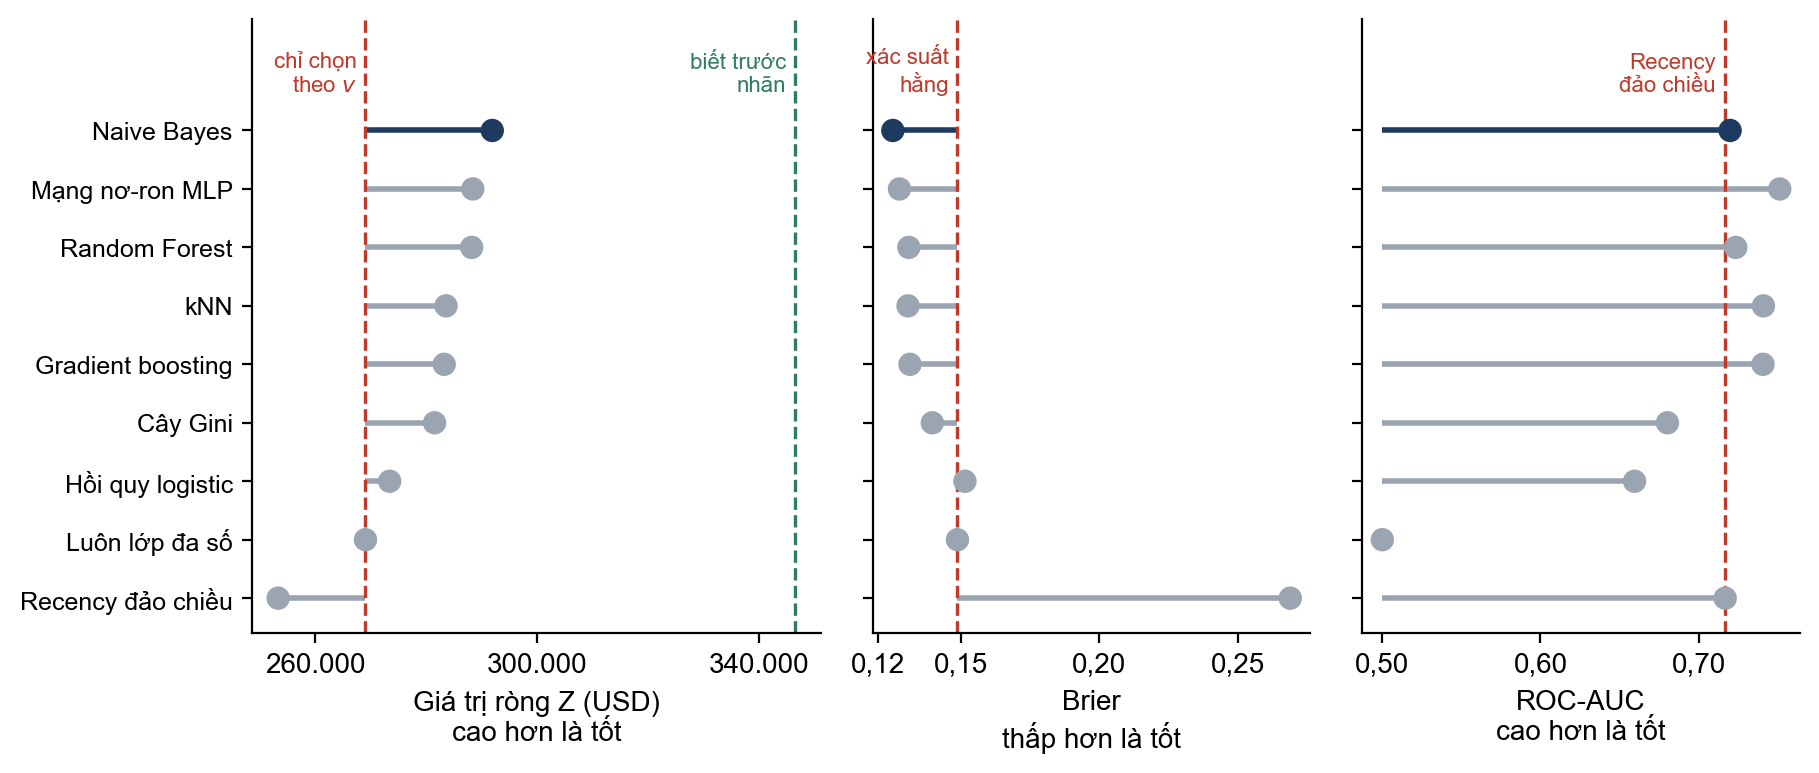
\includegraphics[width=0.95\textwidth]{m_z_mo_hinh.png}
\caption{Ba tiêu chí của chín phương án, trung bình bốn fold}
\label{fig:zmohinh}
\end{figure}

Mạng nơ-ron xếp hạng tốt nhất (ROC-AUC 0,751 so với 0,720), nhưng Naive Bayes có $Z$ cao hơn ở cả bốn mốc, chênh trung bình 3.504 USD, tức 1,2\% (Bảng~\ref{tab:nbmlp}). Theo luật chọn, Naive Bayes thắng. Mạng nơ-ron còn đổi kết quả theo hạt giống khởi tạo: ROC-AUC tại mốc 15/01/2014 dao động từ 0,710 đến 0,769 giữa ba hạt giống, và ở mọi hạt giống $Z$ đều thấp hơn Naive Bayes ở cả bốn mốc (Hình~\ref{fig:nbmlpseed}). Naive Bayes là mô hình xác định, cho cùng kết quả trên mọi máy.

\begin{table}[!htbp]
\centering
\caption{Giá trị ròng $Z$ (USD) của Naive Bayes và mạng nơ-ron tại từng mốc đánh giá}
\label{tab:nbmlp}
\footnotesize
\begin{tabular}{lrrr}
\toprule
Mốc đánh giá $E$ & $Z$ Naive Bayes & $Z$ MLP & Chênh lệch \\
\midrule
15/12/2013 & 292.046 & 290.319 & 1.727 \\
15/01/2014 & 293.085 & 290.012 & 3.073 \\
15/02/2014 & 293.156 & 289.820 & 3.336 \\
01/03/2014 & 289.246 & 283.366 & 5.880 \\
Trung bình & 291.883 & 288.379 & 3.504 \\
\bottomrule
\end{tabular}

\end{table}

\begin{figure}[!htbp]
\centering
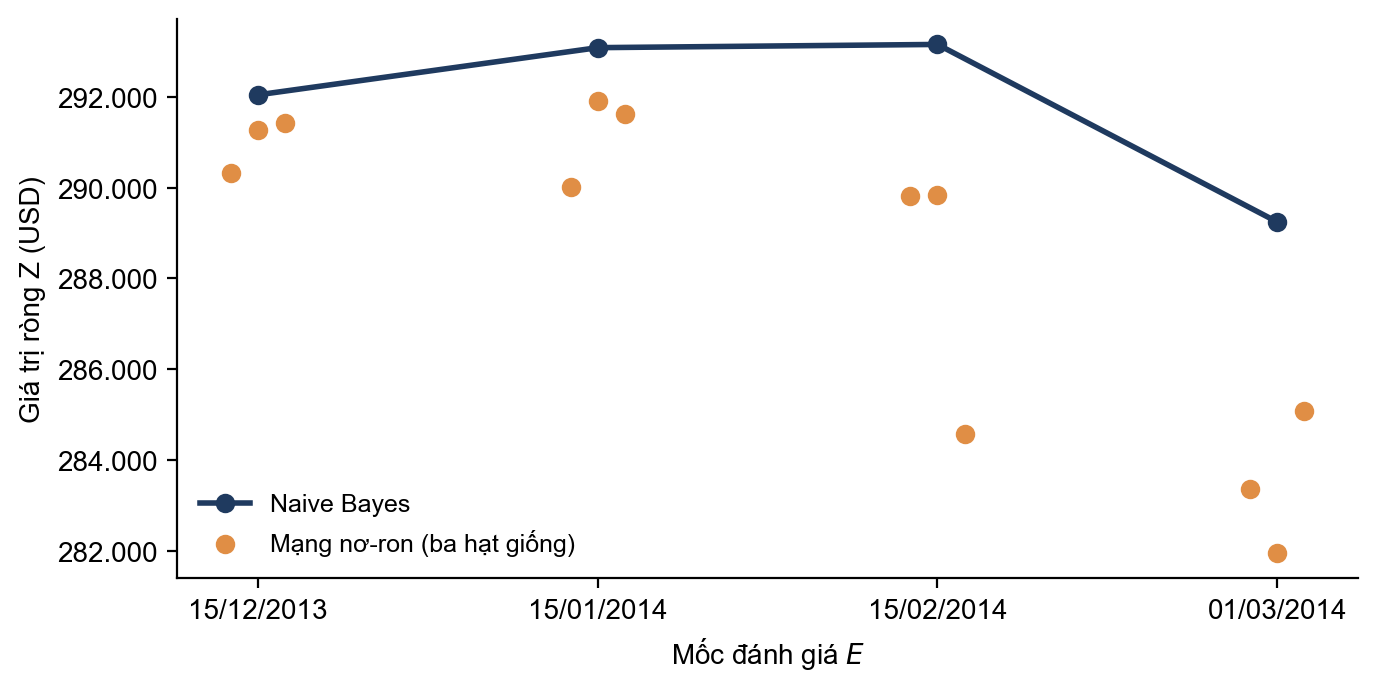
\includegraphics[width=0.7\textwidth]{m_nb_mlp_seed.png}
\caption{Giá trị ròng $Z$ của Naive Bayes và mạng nơ-ron với ba hạt giống}
\label{fig:nbmlpseed}
\end{figure}

Quy tắc Recency đảo chiều xếp hạng gần bằng Naive Bayes (0,717 so với 0,720) nhưng Brier tới 0,269, nên không đạt ĐK2 ở fold nào. Hồi quy logistic có ROC-AUC 0,659, thấp hơn cả quy tắc Recency. Random Forest, gradient boosting và kNN xếp hạng tốt hơn Naive Bayes (ROC-AUC từ 0,724 đến 0,741) nhưng $Z$ không cao hơn. Với bài toán này, xác suất sát thực tế quan trọng hơn khả năng xếp hạng.

\subsubsection{Cây đối chứng: vì sao không dùng để chấm điểm}
Cây Gini đạt điều kiện về $Z$ ở 4/4 fold nhưng ROC-AUC chỉ 0,680 và thấp hơn quy tắc Recency ở 3/4 fold. Nguyên nhân là cây chỉ có 9 đến 11 lá, nên xác suất thô và nhóm nhỏ không tách được thành lá riêng. Vì vậy cây không chấm điểm mà sinh luật IF--THEN để mô tả nhóm khách (mục~\ref{sec:giaithich}). Nút gốc luôn là Recency với ngưỡng từ 131,5 đến 170,5 ngày ở cả bốn mốc, nên luật nhất quán giữa các kỳ.

\subsubsection{Xem kỹ Naive Bayes tại fold cuối}
Phần này xem kỹ Naive Bayes ở fold cuối ($E = 01/03/2014$, học tại $T = 15/11/2013$). Bảng~\ref{tab:lop1} và Hình~\ref{fig:matran} cho ma trận nhầm lẫn và các chỉ số của môn học~\cite{han2011} ở ba cách đặt ngưỡng, cùng cách luôn dự đoán $y=1$ để làm mốc. Ngưỡng Youden~\cite{youden1950} là ngưỡng làm tổng sensitivity (tức recall ở Chương 2) và specificity lớn nhất.

\begin{table}[!htbp]
\centering
\caption{Ma trận nhầm lẫn và chỉ số phân lớp của Naive Bayes tại mốc 01/03/2014}
\label{tab:lop1}
\footnotesize
\resizebox{\textwidth}{!}{\begin{tabular}{lrrrr}
\toprule
Chỉ số & Youden, mốc huấn luyện & Youden, ngoài mẫu & Mức Cao của DSS & Luôn $y=1$ \\
\midrule
Số khách dự đoán $y=1$ & 11.650 & 9.125 & 3.544 & 14.167 \\
Tỷ lệ khách dự đoán $y=1$ & 82,2\% & 64,4\% & 25,0\% & 100,0\% \\
TP & 10.477 & 8.171 & 3.182 & 11.612 \\
FN & 1.135 & 3.441 & 8.430 & 0 \\
FP & 1.173 & 954 & 362 & 2.555 \\
TN & 1.382 & 1.601 & 2.193 & 0 \\
Accuracy & 0,837 & 0,690 & 0,379 & 0,820 \\
Tỷ lệ lỗi (error rate) & 0,163 & 0,310 & 0,621 & 0,180 \\
Precision & 0,899 & 0,895 & 0,898 & 0,820 \\
Sensitivity (recall) & 0,902 & 0,704 & 0,274 & 1,000 \\
Specificity & 0,541 & 0,627 & 0,858 & 0,000 \\
F1 & 0,901 & 0,788 & 0,420 & 0,901 \\
\bottomrule
\end{tabular}
}
\end{table}

\begin{figure}[!htbp]
\centering
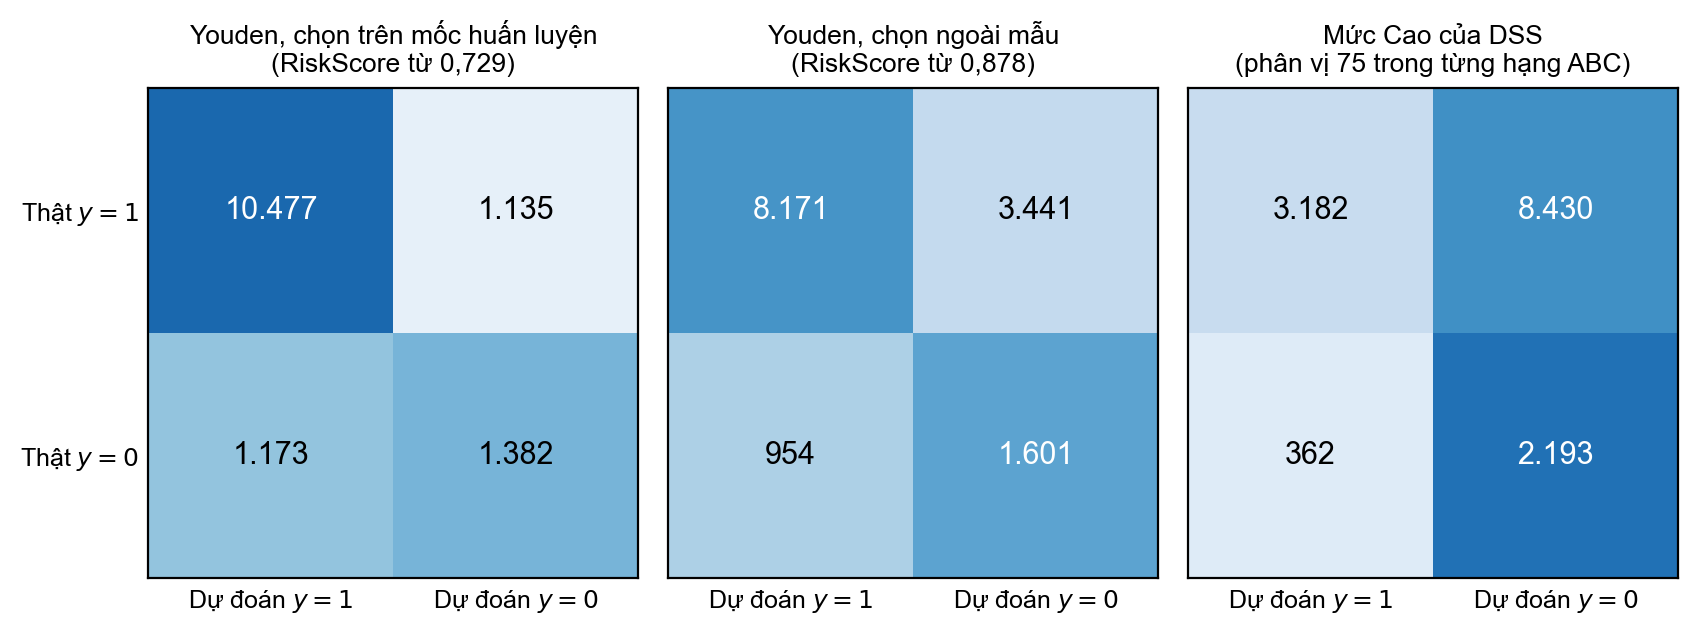
\includegraphics[width=0.95\textwidth]{m_ma_tran.png}
\caption{Ma trận nhầm lẫn của Naive Bayes ở ba cách đặt ngưỡng}
\label{fig:matran}
\end{figure}

Ngưỡng Youden chọn trên mốc huấn luyện cảnh báo 82,2\% số khách, đạt accuracy 0,837 và F1 0,901. Con số đẹp này là do lớp $y=1$ chiếm 82,0\% số khách: cách luôn dự đoán $y=1$ cũng đạt accuracy 0,820 và F1 0,901 nhưng specificity bằng 0. Vì vậy accuracy và F1 không dùng được một mình khi lớp mục tiêu chiếm đa số. Ngưỡng Youden chọn ngoài mẫu (trên mốc 15/11/2013) chỉ cảnh báo 64,4\% khách và cân bằng hơn hẳn (sensitivity 0,704, specificity 0,627), cho thấy ngưỡng chọn trên chính mốc huấn luyện là lạc quan.

Mức Cao của DSS (phân vị 75 trong từng hạng ABC) chỉ cảnh báo 25,0\% khách, nên sensitivity thấp theo chủ ý. Điều quan trọng là precision đạt 0,898 so với tỷ lệ nền 0,820: trong 10 khách mức Cao có khoảng 9 khách thật sự không mua lại, và specificity 0,858 nghĩa là ít khách sẽ mua lại bị làm phiền. Mức Cao là danh sách ưu tiên chứ không phải bộ phát hiện đầy đủ: nó có ít cảnh báo sai nhất (362 khách) nhưng bỏ sót nhiều khách $y=1$ nhất (8.430 khách). Nhóm không gắn mức Cao vẫn có 79,4\% khách $y=1$, chỉ thấp hơn tỷ lệ nền 2,6 điểm phần trăm, nên mô hình tách hai nhóm khách ở mức vừa phải, phù hợp với ROC-AUC 0,72.

Bảng~\ref{tab:lop23} cho hai nhóm chỉ số còn lại: chất lượng xác suất và giá trị quyết định. ROC-AUC của Naive Bayes (0,7207) chỉ nhỉnh hơn Recency đảo chiều (0,7191), đây là điểm yếu cần thừa nhận. Giá trị của mô hình nằm ở xác suất: Brier đạt 0,1176 so với 0,1480 của cách gán xác suất hằng. Khi chọn theo $p \cdot v$, $Z$ đạt 289.245,54 USD, cao hơn 13,7\% so với 254.292,63 USD khi chỉ chọn theo $v$, và lấp được khoảng 41\% khoảng cách từ mức đó đến mức trần 339.886,26 USD khi biết trước nhãn. Nói cách khác, Recency đủ để biết ai có nguy cơ, nhưng cần xác suất tốt để quyết định chi ngân sách cho ai. Hình~\ref{fig:rocpr} vẽ đường ROC (tỷ lệ bắt đúng khách $y=1$ theo tỷ lệ báo nhầm khách $y=0$ khi ngưỡng thay đổi, diện tích dưới đường là ROC-AUC) và cho thấy đường của Naive Bayes và Recency đảo chiều gần trùng nhau, mạng nơ-ron cao hơn ở vùng giữa, còn cây có dạng bậc thang vì chỉ có 11 mức xác suất. Đường Precision--Recall được vẽ thêm vì lớp $y=1$ chiếm khoảng 82\%~\cite{saito2015}.

\begin{table}[!htbp]
\centering
\caption{Chất lượng điểm và giá trị quyết định của Naive Bayes tại mốc 01/03/2014}
\label{tab:lop23}
\footnotesize
\begin{tabular}{llr}
\toprule
Lớp & Chỉ số & Giá trị tại mốc 01/03/2014 \\
\midrule
Xếp hạng & ROC-AUC của Naive Bayes & 0,7207 \\
 & ROC-AUC của Recency đảo chiều & 0,7191 \\
 & Average precision, lớp $y=1$ & 0,893 \\
 & Average precision, lớp $y=0$ & 0,476 \\
 & Precision@4.000 & 89,33\% \\
Chất lượng xác suất & Brier của Naive Bayes & 0,1176 \\
 & Brier của cách dự đoán một xác suất hằng & 0,1480 \\
Giá trị quyết định & $Z$ khi chọn theo $p\cdot v$ (USD) & 289.245,54 \\
 & $Z$ khi chỉ chọn theo $v$ (USD) & 254.292,63 \\
 & $Z$ khi biết trước nhãn (USD) & 339.886,26 \\
\bottomrule
\end{tabular}

\end{table}

\begin{figure}[!htbp]
\centering
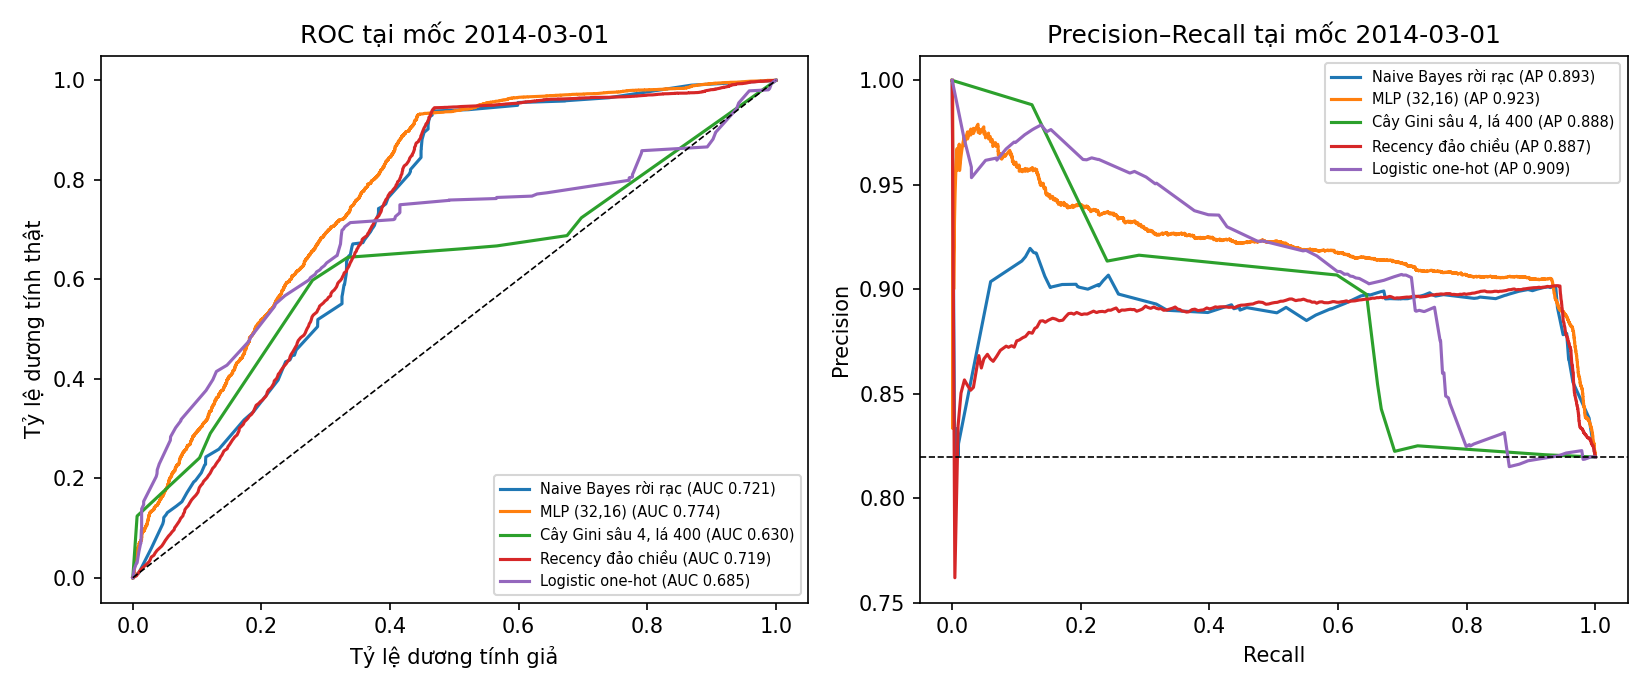
\includegraphics[width=\textwidth]{m_roc_pr.png}
\caption{Đường ROC (trái) và Precision--Recall (phải) tại mốc 01/03/2014}
\label{fig:rocpr}
\end{figure}

\subsubsection{Nhãn 90 ngày và nhãn 180 ngày}\label{sec:nhan180}
Nhãn $y=1$ gồm cả khách đã bỏ đi lẫn khách chưa đến kỳ mua lại. Để đo mức nhiễu này, nhóm so nhãn 90 ngày với nhãn 180 ngày ở 13 mốc từ 01/06/2013 đến 01/12/2013, là các mốc có cửa sổ 180 ngày đã khép (Bảng~\ref{tab:nhan180}). Tỷ lệ $y=1$ trung bình giảm từ 80,8\% xuống 59,6\%. Trong số khách bị gắn $y=1$ theo nhãn 90 ngày, 26,2\% có mua lại trong ngày 90 đến 180, tức khoảng một phần tư là khách chưa đến kỳ chứ chưa bỏ đi. Khi đối chiếu điểm của mô hình học theo nhãn 90 ngày với nhãn 180 ngày ở ba mốc cuối, ROC-AUC trung bình của Naive Bayes tăng từ 0,694 lên 0,752, nghĩa là điểm rủi ro xếp hạng tốt hơn với hành vi không mua lại kéo dài. Quy tắc Recency tăng tương tự (0,693 lên 0,759), cây tăng ít hơn (0,653 lên 0,678).

\begin{table}[!htbp]
\centering
\caption{Tỷ lệ $y=1$ theo nhãn 90 ngày và 180 ngày tại các mốc có đủ cửa sổ 180 ngày}
\label{tab:nhan180}
\footnotesize
\begin{tabular}{lR{1.6cm}R{2.0cm}R{2.0cm}R{3.6cm}R{2.2cm}}
\toprule
Mốc $T$ & Số khách & $y=1$ (90 ngày) & $y=1$ (180 ngày) & Khách $y=1$ mua lại trong ngày 90--180 & Tỷ lệ chưa đến kỳ \\
\midrule
01/06/2013 & 5.324 & 82,8\% & 60,1\% & 1.205 & 27,4\% \\
15/06/2013 & 5.423 & 82,6\% & 59,1\% & 1.271 & 28,4\% \\
01/07/2013 & 5.536 & 82,2\% & 57,5\% & 1.363 & 30,0\% \\
15/07/2013 & 5.889 & 82,0\% & 57,2\% & 1.457 & 30,2\% \\
01/08/2013 & 6.529 & 81,5\% & 57,6\% & 1.563 & 29,4\% \\
15/08/2013 & 7.077 & 80,3\% & 58,3\% & 1.555 & 27,4\% \\
01/09/2013 & 7.705 & 79,5\% & 59,1\% & 1.572 & 25,7\% \\
15/09/2013 & 8.249 & 79,6\% & 59,7\% & 1.640 & 25,0\% \\
01/10/2013 & 8.812 & 79,4\% & 59,9\% & 1.720 & 24,6\% \\
15/10/2013 & 9.305 & 79,3\% & 60,0\% & 1.795 & 24,3\% \\
01/11/2013 & 9.898 & 79,4\% & 60,8\% & 1.835 & 23,4\% \\
15/11/2013 & 10.447 & 80,7\% & 62,5\% & 1.899 & 22,5\% \\
01/12/2013 & 11.055 & 81,4\% & 63,4\% & 1.986 & 22,1\% \\
\bottomrule
\end{tabular}

\end{table}

Nhóm không huấn luyện thẳng một mô hình với nhãn 180 ngày, vì khi đó mốc huấn luyện phải trước 01/06/2013, mà tại đó mọi khách chỉ có một đơn, đều đã mua xe đạp và có $NSub = 1$ nên không có gì để học. Vì vậy nhãn 90 ngày được giữ, và \texttt{RiskScore} cần hiểu là khả năng không mua lại trong kỳ tới, không phải xác suất khách đã rời bỏ hẳn.

\subsubsection{Kết luận chọn mô hình và giới hạn}
Naive Bayes là mô hình chấm điểm vì đạt cả ba điều kiện ở 4/4 fold và có $Z$ cao hơn mạng nơ-ron ở 4/4 mốc. Cây Gini giữ vai trò đối chứng và sinh luật, mạng nơ-ron chỉ để so sánh. Có ba giới hạn cần nhớ. Bốn fold có cửa sổ nhãn chồng nhau và cấu hình cũng được chọn trên chính bốn fold này, nên kết quả có thiên lệch lựa chọn. Chênh lệch $Z$ giữa Naive Bayes và mạng nơ-ron (1,2\%) nhỏ hơn mức dao động của mạng nơ-ron giữa các hạt giống, nên Naive Bayes được chọn vì thắng nhất quán ở mọi mốc và mọi hạt giống, không vì độ lớn của chênh lệch. Khả năng xếp hạng chỉ ngang quy tắc Recency, nên lợi thế của mô hình đến từ chất lượng xác suất.

\subsection{Giải thích dự đoán}\label{sec:giaithich}
Người ra quyết định cần biết vì sao một khách bị chấm điểm cao. Nhóm giải thích ở hai tầng: tầng một cho biết thuộc tính nào kéo xác suất lên hay xuống, tầng hai mô tả khách thuộc nhóm nào.

\subsubsection{Tầng một: xác suất có điều kiện của Naive Bayes}
Bảng~\ref{tab:xacsuat} và Hình~\ref{fig:tysonb} cho xác suất của từng giá trị thuộc tính trong mỗi lớp, ước lượng trên mốc 01/03/2014. Tỷ số $P(x \mid y=1)/P(x \mid y=0)$ lớn hơn 1 nghĩa là giá trị đó làm tăng rủi ro. Recency chi phối: Recency từ 180 đến 269 ngày có tỷ số 2,495, tăng rủi ro mạnh nhất, còn Recency từ 270 đến 539 ngày có tỷ số 0,09 đến 0,10, giảm rủi ro rất mạnh. Điều này khớp với Hình~\ref{fig:ytheokhoang}: nhóm sau chủ yếu là khách của đợt tăng vọt tháng 7/2013 nay đã đến kỳ mua lại. Monetary thấp (Q1) có tỷ số 1,907, NSub bằng 2 có 2,748. Hai thuộc tính Monetary và BikeBuyer phụ thuộc mạnh nên Naive Bayes đếm hai lần cùng thông tin ``đã mua xe đắt'', không cộng dồn hai dòng này khi diễn giải. Trong cây đối chứng, độ quan trọng Gini của Recency là 0,83 và của Monetary là 0,12, còn NSub bằng 0 vì cây sâu 4 đã dùng hết các phép tách cho hai thuộc tính trước. Giá trị của NSub chỉ thể hiện qua Naive Bayes (Bảng~\ref{tab:tapthuoctinh}).

\begin{table}[!htbp]
\centering
\caption{Xác suất có điều kiện của Naive Bayes tại mốc huấn luyện 01/03/2014}
\label{tab:xacsuat}
\footnotesize
\begin{tabular}{llrrr}
\toprule
Thuộc tính & Khoảng & $P(x\mid y=0)$ & $P(x\mid y=1)$ & Tỷ số \\
\midrule
Recency & $<$90 & 20,4\% & 36,1\% & 1,77 \\
 & 90--179 & 17,0\% & 34,9\% & 2,06 \\
 & 180--269 & 9,2\% & 23,0\% & 2,50 \\
 & 270--364 & 13,5\% & 1,4\% & 0,10 \\
 & 365--539 & 13,2\% & 1,2\% & 0,09 \\
 & $\geq$540 & 26,8\% & 3,4\% & 0,13 \\
Frequency & 1 & 75,8\% & 67,9\% & 0,90 \\
 & 2 & 19,9\% & 27,5\% & 1,38 \\
 & $\geq$3 & 4,2\% & 4,6\% & 1,09 \\
Monetary & Q1 (thấp nhất) & 14,4\% & 27,5\% & 1,91 \\
 & Q2 & 13,6\% & 27,4\% & 2,01 \\
 & Q3 & 43,6\% & 20,9\% & 0,48 \\
 & Q4 (cao nhất) & 28,3\% & 24,2\% & 0,85 \\
BikeBuyer & 0 & 28,8\% & 49,7\% & 1,73 \\
 & 1 & 71,2\% & 50,3\% & 0,71 \\
NSub & 1 & 66,0\% & 28,2\% & 0,43 \\
 & 2 & 13,4\% & 36,7\% & 2,75 \\
 & 3--4 & 16,6\% & 30,6\% & 1,84 \\
 & $\geq$5 & 4,0\% & 4,5\% & 1,13 \\
\bottomrule
\end{tabular}

\end{table}

\begin{figure}[!htbp]
\centering
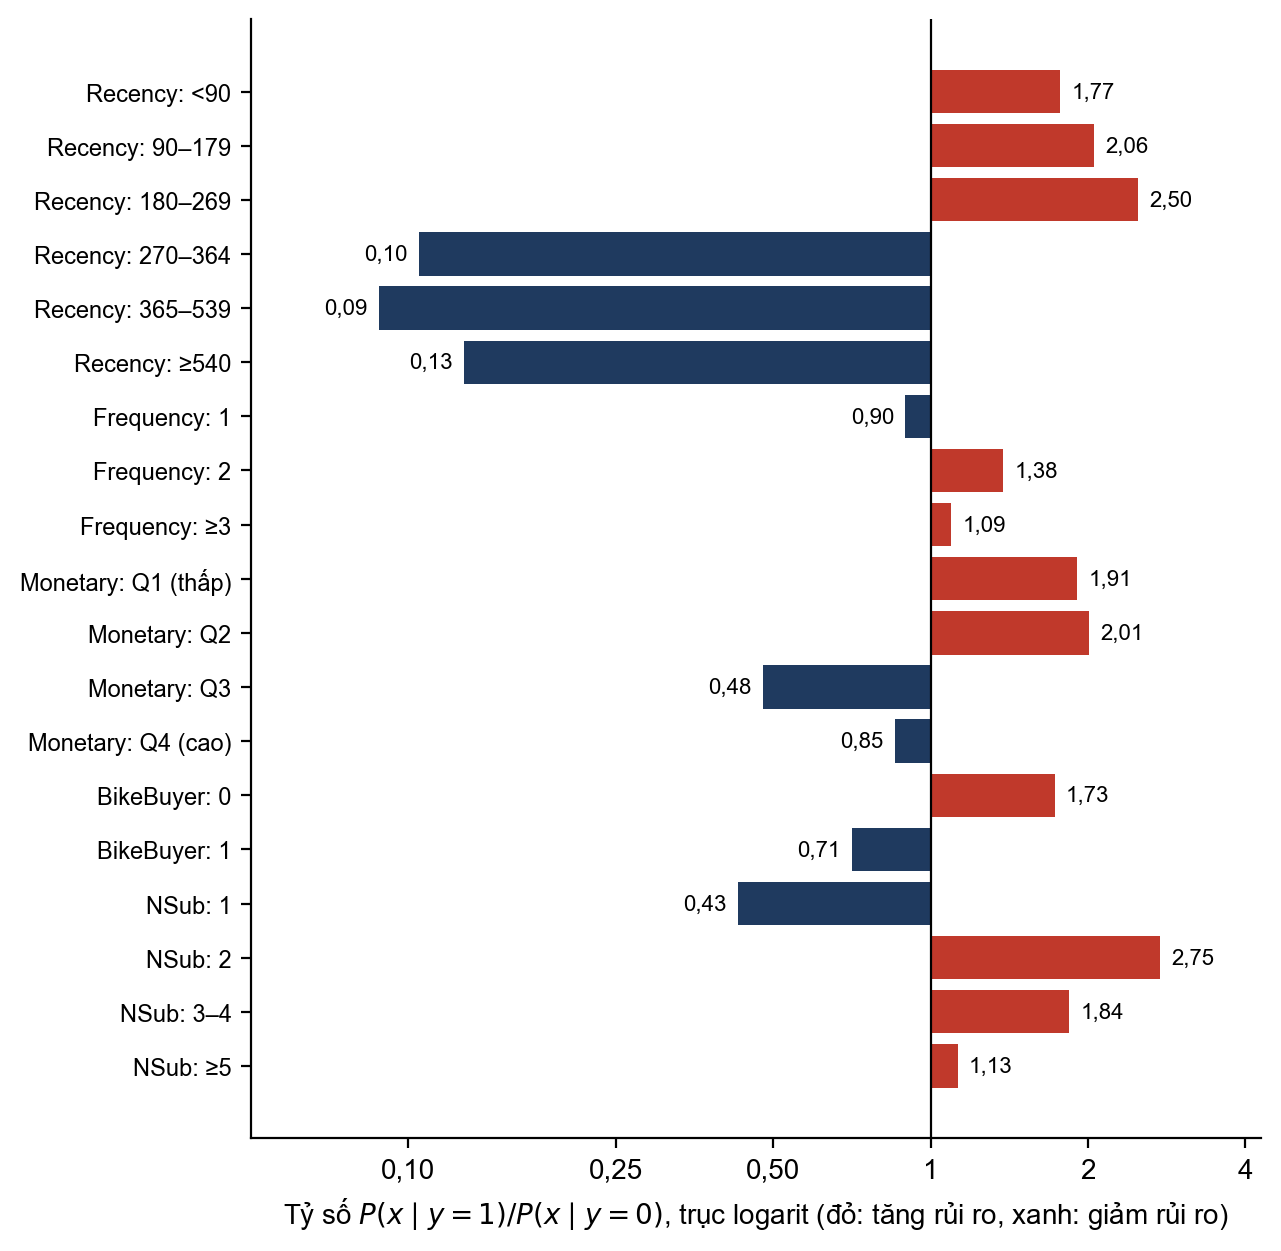
\includegraphics[width=0.62\textwidth]{m_ty_so_nb.png}
\caption{Tỷ số xác suất có điều kiện của Naive Bayes theo khoảng thuộc tính}
\label{fig:tysonb}
\end{figure}

\subsubsection{Tầng hai: luật của cây đối chứng}
Cây học trên mốc 01/03/2014 có 11 lá (Bảng~\ref{tab:lacay}), trong đó 6 lá có tỷ lệ $y=1$ thấp hơn tỷ lệ chung 82,0\%. Mỗi lá là một luật mô tả một nhóm khách giống nhau, kèm tỷ lệ $y=1$ của nhóm và \texttt{TreeScore}, là xác suất của lá sau làm trơn. Đây là mô tả nhóm, không phải lý do tính ra \texttt{RiskScore}. Nhóm có tỷ lệ $y=1$ thấp nhất là lá 8 (Recency trên 275,5 ngày, Tenure không quá 744 ngày, Monetary không quá 1.684,87 USD) với 18,1\%: khách đã lâu không mua nhưng hầu hết vẫn quay lại. DSS hiển thị luật thành câu tiếng Việt, ví dụ ``lần mua gần nhất cách đây trên 275 ngày, đã là khách không quá 744 ngày''.

\begin{table}[!htbp]
\centering
\caption{Các lá của cây đối chứng học tại mốc 01/03/2014 (14.167 khách)}
\label{tab:lacay}
\footnotesize
\begin{tabular}{cp{8.6cm}rrr}
\toprule
Lá & Luật (IF) & Số khách & $y=1$ thô & TreeScore \\
\midrule
1 & Recency $\leq$ 275,5, Monetary $\leq$ 4.640,88, chưa mua xe đạp, Monetary $\leq$ 150,94 & 6.054 & 89,9\% & 0,898 \\
2 & Recency $\leq$ 275,5, Monetary $\leq$ 4.640,88, chưa mua xe đạp, Monetary $>$ 150,94 & 452 & 73,2\% & 0,741 \\
3 & Recency $\leq$ 275,5, Monetary $\leq$ 4.640,88, đã mua xe đạp, Monetary $\leq$ 1.956,81 & 1.756 & 99,5\% & 0,990 \\
4 & Recency $\leq$ 275,5, Monetary $\leq$ 4.640,88, đã mua xe đạp, Monetary $>$ 1.956,81 & 1.904 & 94,6\% & 0,943 \\
5 & Recency $\leq$ 275,5, Monetary từ 4.640,88 đến 4.960,65 & 440 & 55,9\% & 0,586 \\
6 & Recency $\leq$ 275,5, Monetary từ 4.960,65 đến 6.587,16 & 901 & 86,1\% & 0,859 \\
7 & Recency $\leq$ 275,5, Monetary $>$ 6.587,16 & 664 & 95,2\% & 0,943 \\
8 & Recency $>$ 275,5, Tenure $\leq$ 744, Monetary $\leq$ 1.684,87 & 420 & 18,1\% & 0,249 \\
9 & Recency $>$ 275,5, Tenure $\leq$ 744, Monetary từ 1.684,87 đến 2.349,77 & 467 & 37,5\% & 0,418 \\
10 & Recency $>$ 275,5, Tenure $\leq$ 744, Monetary $>$ 2.349,77 & 515 & 20,2\% & 0,257 \\
11 & Recency $>$ 275,5, Tenure $>$ 744 & 594 & 47,8\% & 0,505 \\
\bottomrule
\end{tabular}

\end{table}

\subsubsection{Cờ lệch giữa hai mô hình}
Khi \texttt{RiskScore} và \texttt{TreeScore} chênh nhau quá 0,3, khách được gắn cờ ``cần xem xét thêm''. Cờ không đổi điểm, chỉ báo cho người quản lý rằng hai mô hình không thống nhất. Trong 18.360 khách chấm điểm có 2.560 khách (13,9\%) bị gắn cờ, tập trung ở lá 8 (1.376 trên 2.727 khách), vì \texttt{RiskScore} trung bình của họ là 0,55 trong khi \texttt{TreeScore} chỉ 0,25. Bảng~\ref{tab:minhhoa} minh hoạ ba khách điển hình.
\begin{itemize}
    \item \textbf{Khách 12201} (hạng C, Recency 180 ngày, 2 đơn, 64,29 USD): \texttt{RiskScore} 0,993, thuộc lá 1 (89,9\% không mua lại). Hai mô hình thống nhất.
    \item \textbf{Khách 26339} (hạng A, Recency 186 ngày, 2 đơn, 4.923,32 USD): \texttt{RiskScore} 0,963, mức Cao, nhưng thuộc lá 5 có \texttt{TreeScore} 0,586. Chênh lệch 0,377 vượt 0,3 nên bị gắn cờ.
    \item \textbf{Khách 26774} (hạng C, Recency 508 ngày, 1 đơn, 865,20 USD): \texttt{RiskScore} 0,049, mức Thấp, thuộc lá 8 (\texttt{TreeScore} 0,249). Hai mô hình thống nhất rằng khách này nhiều khả năng sẽ quay lại.
\end{itemize}

\begin{table}[!htbp]
\centering
\caption{Ba khách minh hoạ tại mốc chấm điểm 08/07/2014}
\label{tab:minhhoa}
\footnotesize
\resizebox{\textwidth}{!}{\begin{tabular}{rrrrrrlrcc}
\toprule
Mã khách & Recency & Frequency & Monetary & RiskScore & Phân vị & Mức & TreeScore & Cờ lệch & Lá \\
\midrule
12201 & 180 & 2 & 64,29 & 0,993 & 100,0 & Cao & 0,898 & Không & 1 \\
26339 & 186 & 2 & 4.923,32 & 0,963 & 99,7 & Cao & 0,586 & Có & 5 \\
26774 & 508 & 1 & 865,20 & 0,049 & 0,0 & Thấp & 0,249 & Không & 8 \\
\bottomrule
\end{tabular}
}
\end{table}

\subsection{Chấm điểm và lưu kết quả vào kho}\label{sec:chamdiem}
Kết quả mô hình được đưa trở lại kho để DSS đọc, thay vì để rời trong tệp, qua bốn việc nối tiếp nhau.
\begin{enumerate}
    \item \textbf{Học và chấm điểm.} Python học Naive Bayes và cây trên mốc 01/03/2014, chấm 18.360 khách tại mốc 08/07/2014 rồi sinh các tệp SQL. Script tự kiểm tra: mỗi khách đúng một dòng, \texttt{RiskLevel} khớp phân vị, mỗi hạng ABC có đúng 25\% khách mức Cao.
    \item \textbf{Đăng ký mô hình} vào \texttt{analytics.\allowbreak ModelRegistry} với ba phiên bản: Naive Bayes (chấm điểm), cây (đối chứng) và mạng nơ-ron (so sánh). Một chỉ mục duy nhất có điều kiện bảo đảm chỉ một mô hình chấm điểm đang dùng.
    \item \textbf{Lưu 11 lá của cây} vào \texttt{analytics.\allowbreak ModelTreeLeaf}.
    \item \textbf{Ghi 18.360 dòng điểm} vào \texttt{analytics.\allowbreak CustomerRiskScore} với các cột \texttt{RiskScore}, \texttt{RiskPercentile}, \texttt{RiskLevel}, \texttt{TreeScore}, \texttt{TopFactors} (luật của lá) và thời điểm chấm. Khoá gồm mã khách, ngày chấm và phiên bản mô hình, nên điểm cũ được giữ khi có phiên bản mới.
\end{enumerate}
Mọi tệp SQL chạy trong một transaction (giao dịch cơ sở dữ liệu) và tự dừng nếu số dòng lệch. Sau khi ghi điểm, bảng Snapshot bị khoá không cho tính lại, để điểm và thuộc tính luôn đi cùng nhau. DSS chỉ đọc phiên bản mô hình chấm điểm đang dùng.

\subsubsection{Mức rủi ro tính trong từng hạng ABC}
\texttt{RiskPercentile} là thứ hạng phần trăm của \texttt{RiskScore} trong từng hạng ABC (ba hạng ở Chương 4). Khách có phân vị từ 75 trở lên được gắn mức Cao, khách đồng điểm xếp theo Recency giảm dần. Nhóm tính trong từng hạng chứ không tính chung, vì tính chung thì khách mức Cao dồn vào hạng C và ma trận Rủi ro $\times$ Giá trị ở Chương 6 không còn phân biệt được gì. Hệ quả là không có một ngưỡng \texttt{RiskScore} chung cho mức Cao (Bảng~\ref{tab:hangabc}, hai cột cuối là \texttt{RiskScore} thấp nhất và trung vị của khách mức Cao, và Hình~\ref{fig:diemhang}): \texttt{RiskScore} thấp nhất của khách mức Cao là 0,935 ở hạng A, 0,886 ở hạng B và 0,986 ở hạng C. Cả ba đều cao hơn tỷ lệ nền 0,82, nên khách mức Cao ở hạng nào cũng có xác suất không mua lại cao. Mức rủi ro là thứ tự ưu tiên trong hạng, còn \texttt{RiskScore} mới là xác suất. Trên toàn bộ khách, \texttt{RiskScore} có trung vị 0,922 và hai tứ phân vị 0,803 và 0,975 (Hình~\ref{fig:phanbo_diem}, đường đứt là phân vị 75 của toàn bộ khách, chỉ để tham khảo vì mức Cao tính riêng trong từng hạng).

\begin{table}[!htbp]
\centering
\caption{Kết quả chấm điểm 18.360 khách tại mốc 08/07/2014 theo hạng ABC}
\label{tab:hangabc}
\footnotesize
\begin{tabular}{lrrrrr}
\toprule
Hạng & Số khách & Số khách mức Cao & Tỷ lệ & Thấp nhất & Trung vị \\
\midrule
Hạng A & 5.137 & 1.285 & 25,0\% & 0,935 & 0,946 \\
Hạng B & 2.581 & 646 & 25,0\% & 0,886 & 0,904 \\
Hạng C & 10.642 & 2.661 & 25,0\% & 0,986 & 0,989 \\
Cộng & 18.360 & 4.592 & 25,0\% & -- & -- \\
\bottomrule
\end{tabular}

\end{table}

\begin{figure}[!htbp]
\centering
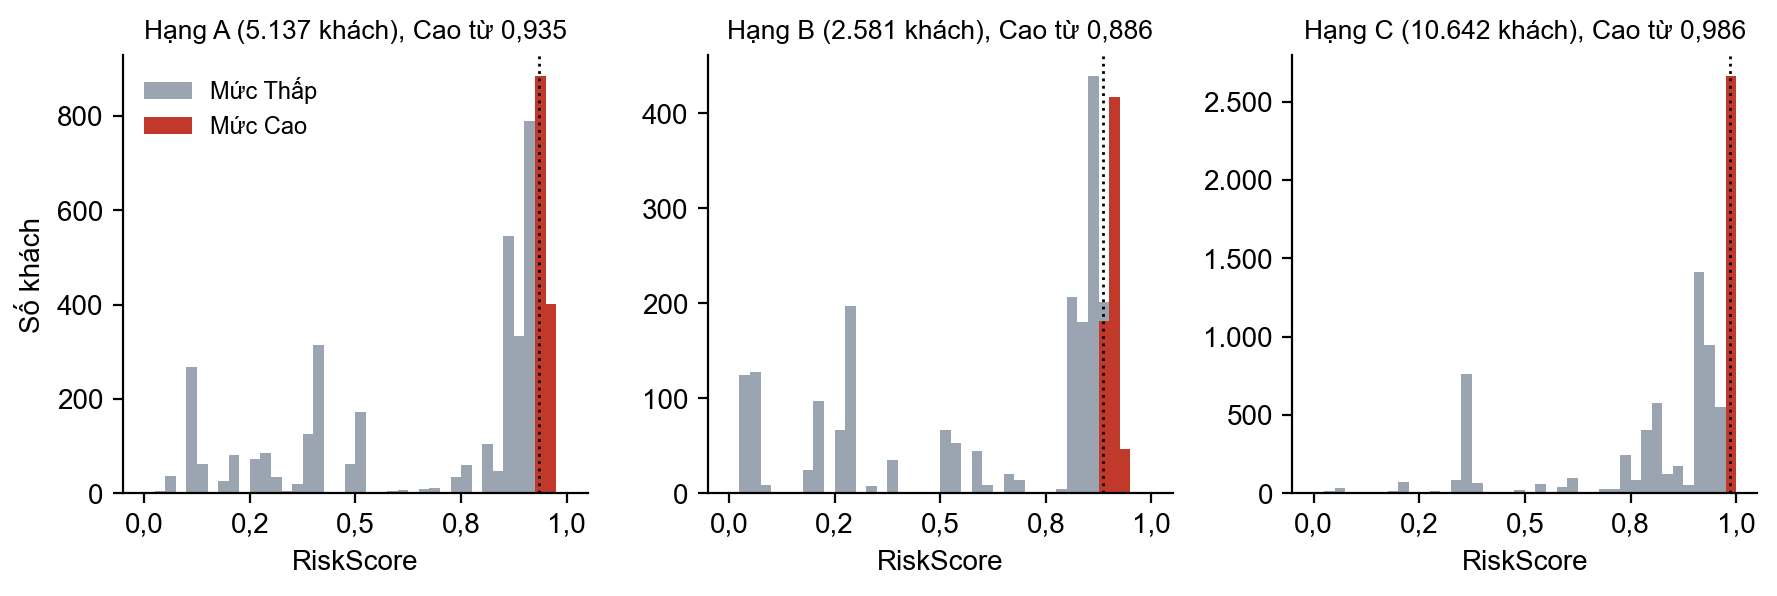
\includegraphics[width=0.95\textwidth]{m_diem_theo_hang.png}
\caption{Phân bố \texttt{RiskScore} của khách mức Cao và mức Thấp theo hạng ABC}
\label{fig:diemhang}
\end{figure}

\begin{figure}[!htbp]
\centering
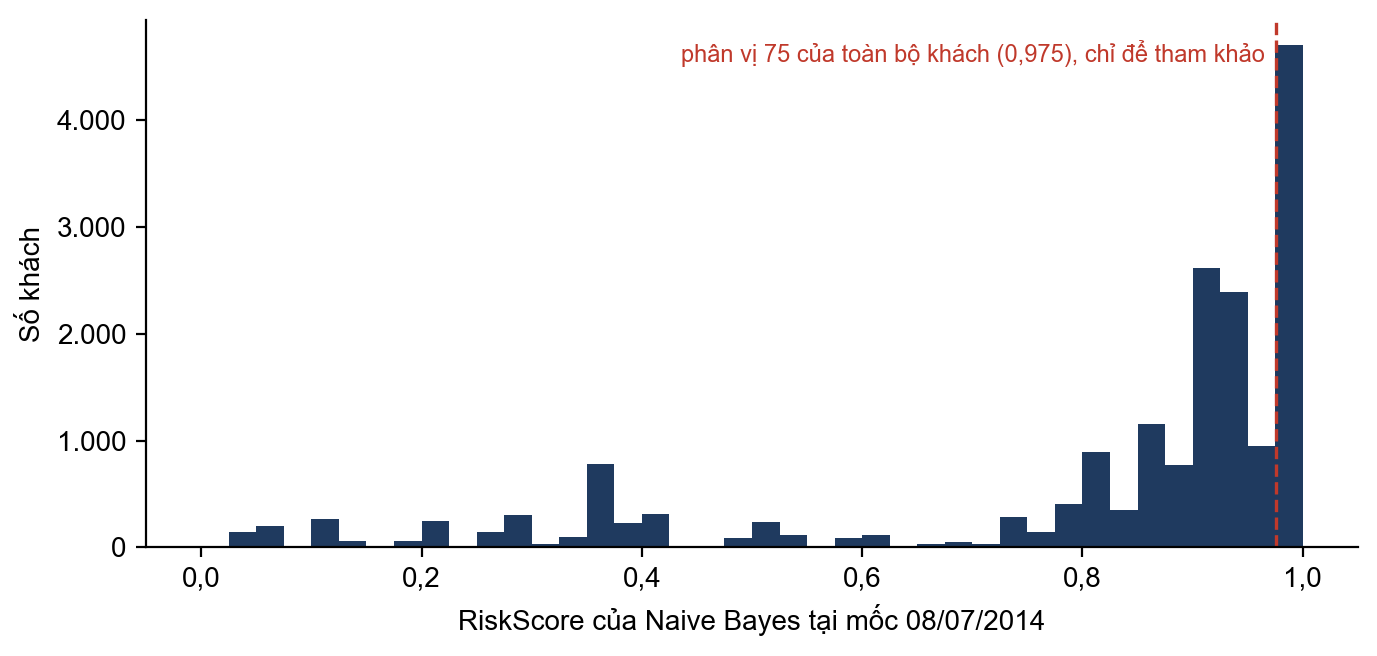
\includegraphics[width=0.55\textwidth]{m_phan_bo_diem.png}
\caption{Phân bố \texttt{RiskScore} trên 18.360 khách tại mốc 08/07/2014}
\label{fig:phanbo_diem}
\end{figure}
\FloatBarrier
